% !TEX root = presentation.tex
%LTeX: language=de-CH


\begin{frame}
\titlepage
\end{frame}

% \begin{frame}
%   \frametitle{Forecast: 01-May-2025 at 00:00, Level 850 hPa}
%   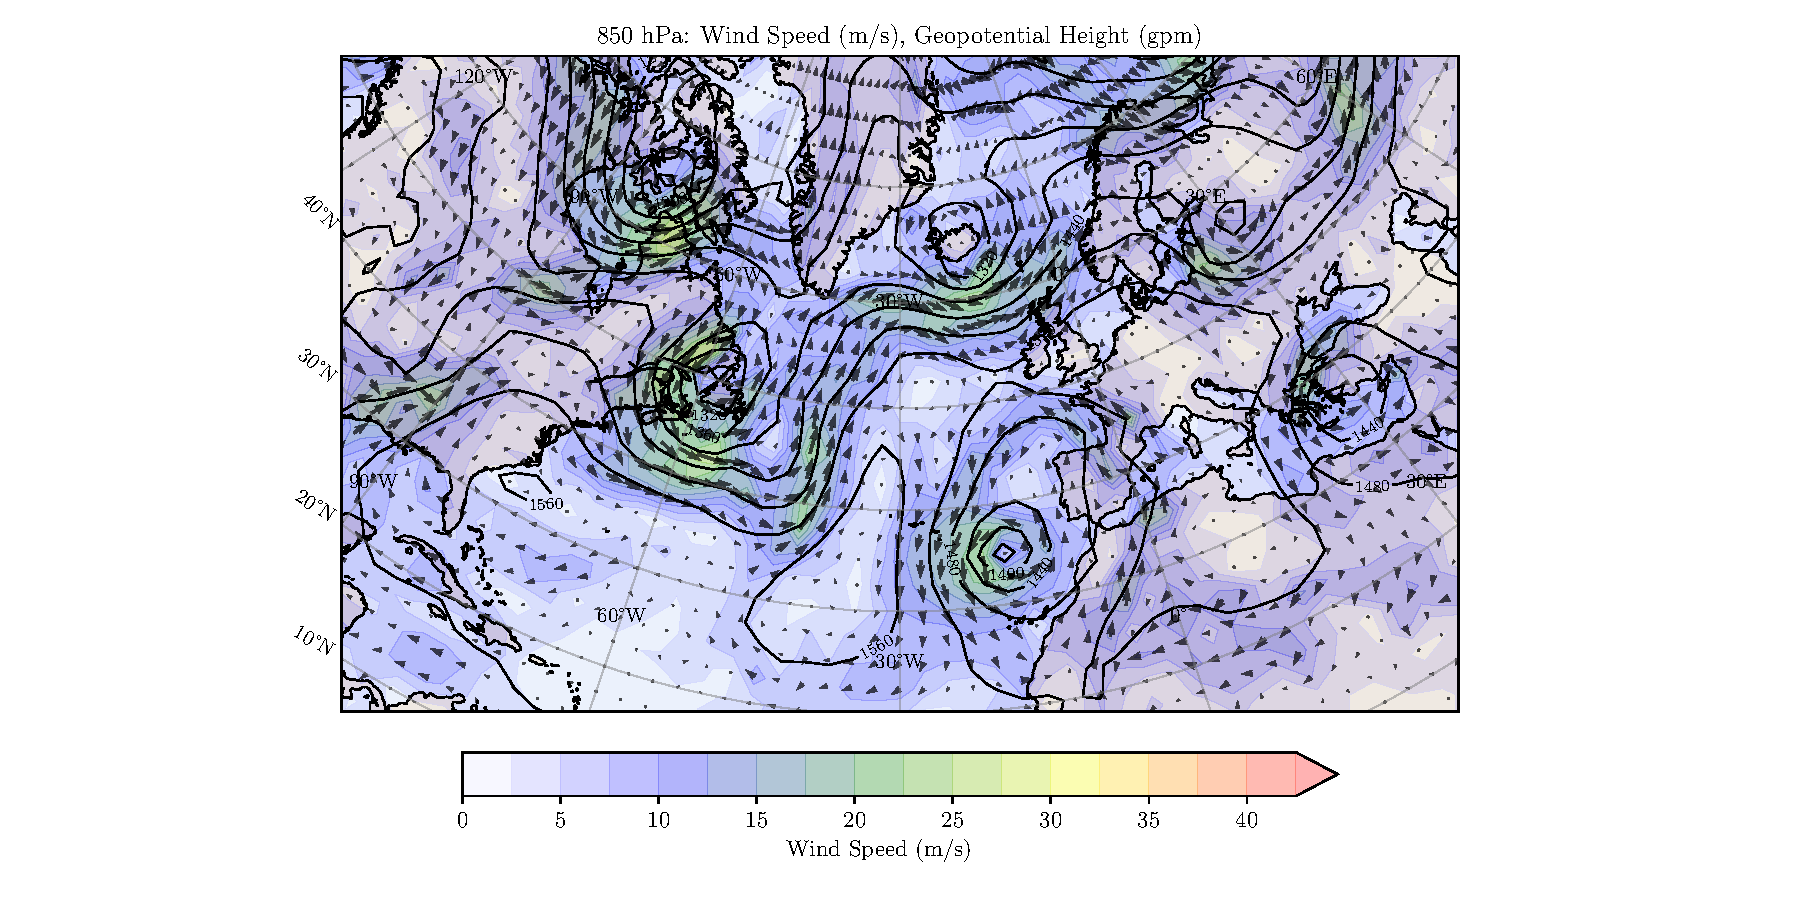
\includegraphics[width=\textwidth]{../images/weather/data_2025_5_1_00:00_850.pdf}
% \end{frame}
% \begin{frame}
%   \frametitle{Forecast: 01-May-2025 at 00:00, Level 500 hPa}
%   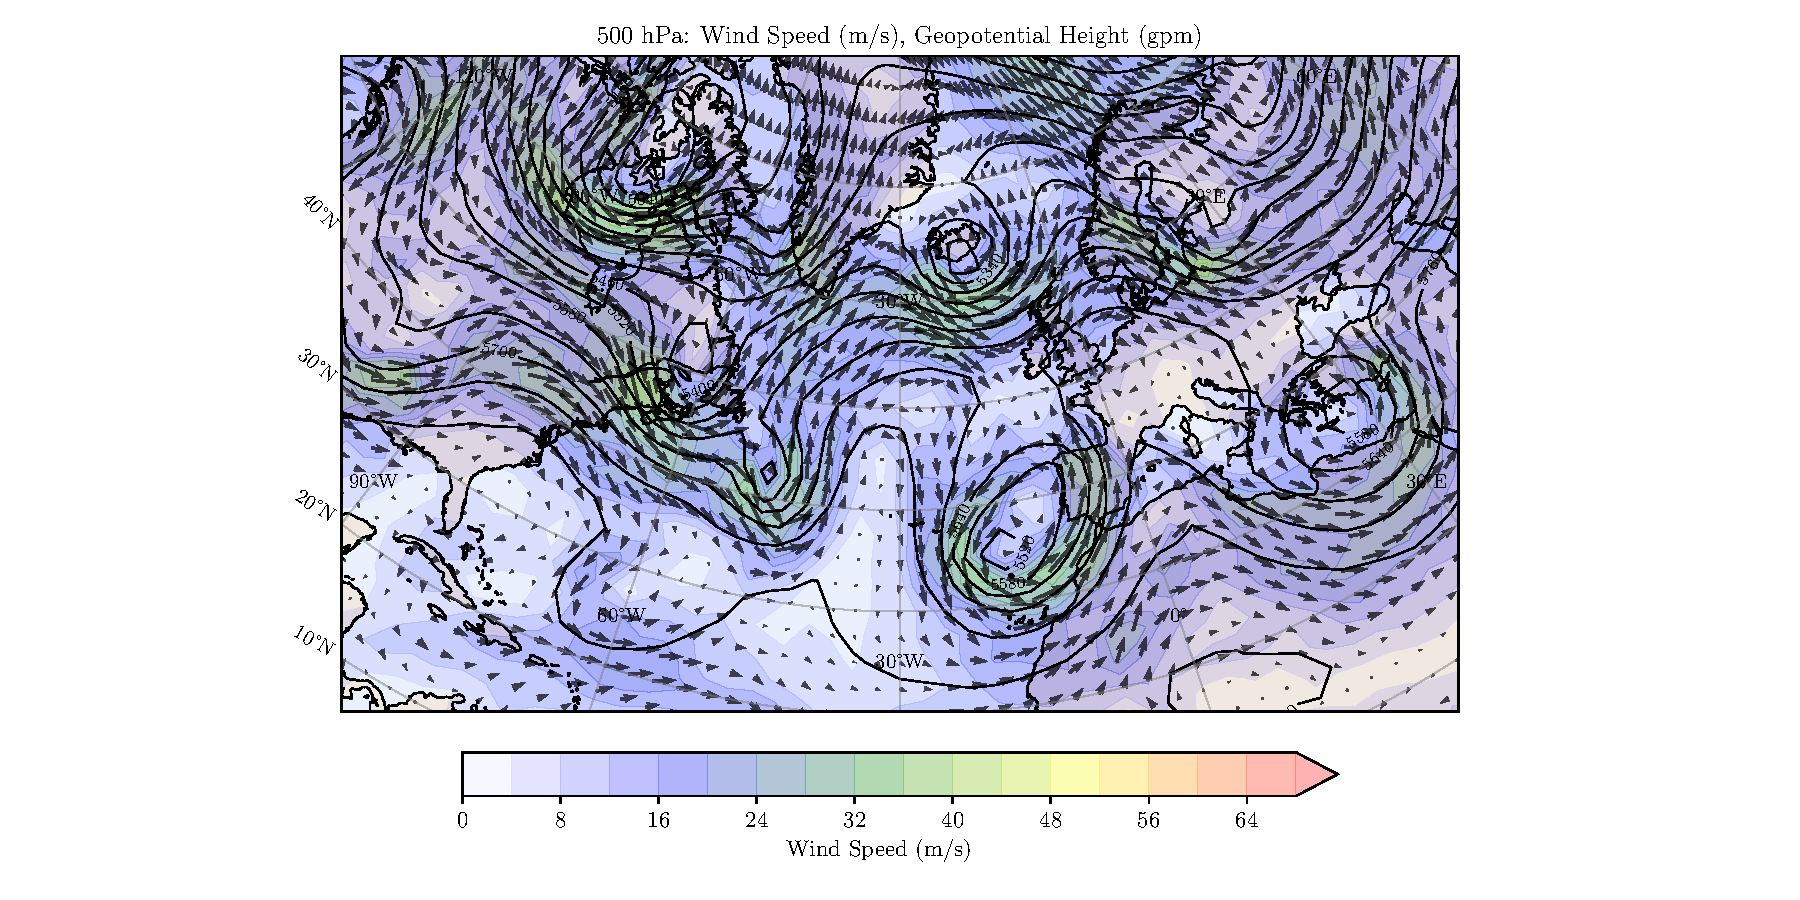
\includegraphics[width=\textwidth]{../images/weather/data_2025_5_1_00:00_500.pdf}
% \end{frame}
% \begin{frame}
%   \frametitle{Forecast: 01-May-2025 at 00:00, Level 200 hPa}
%   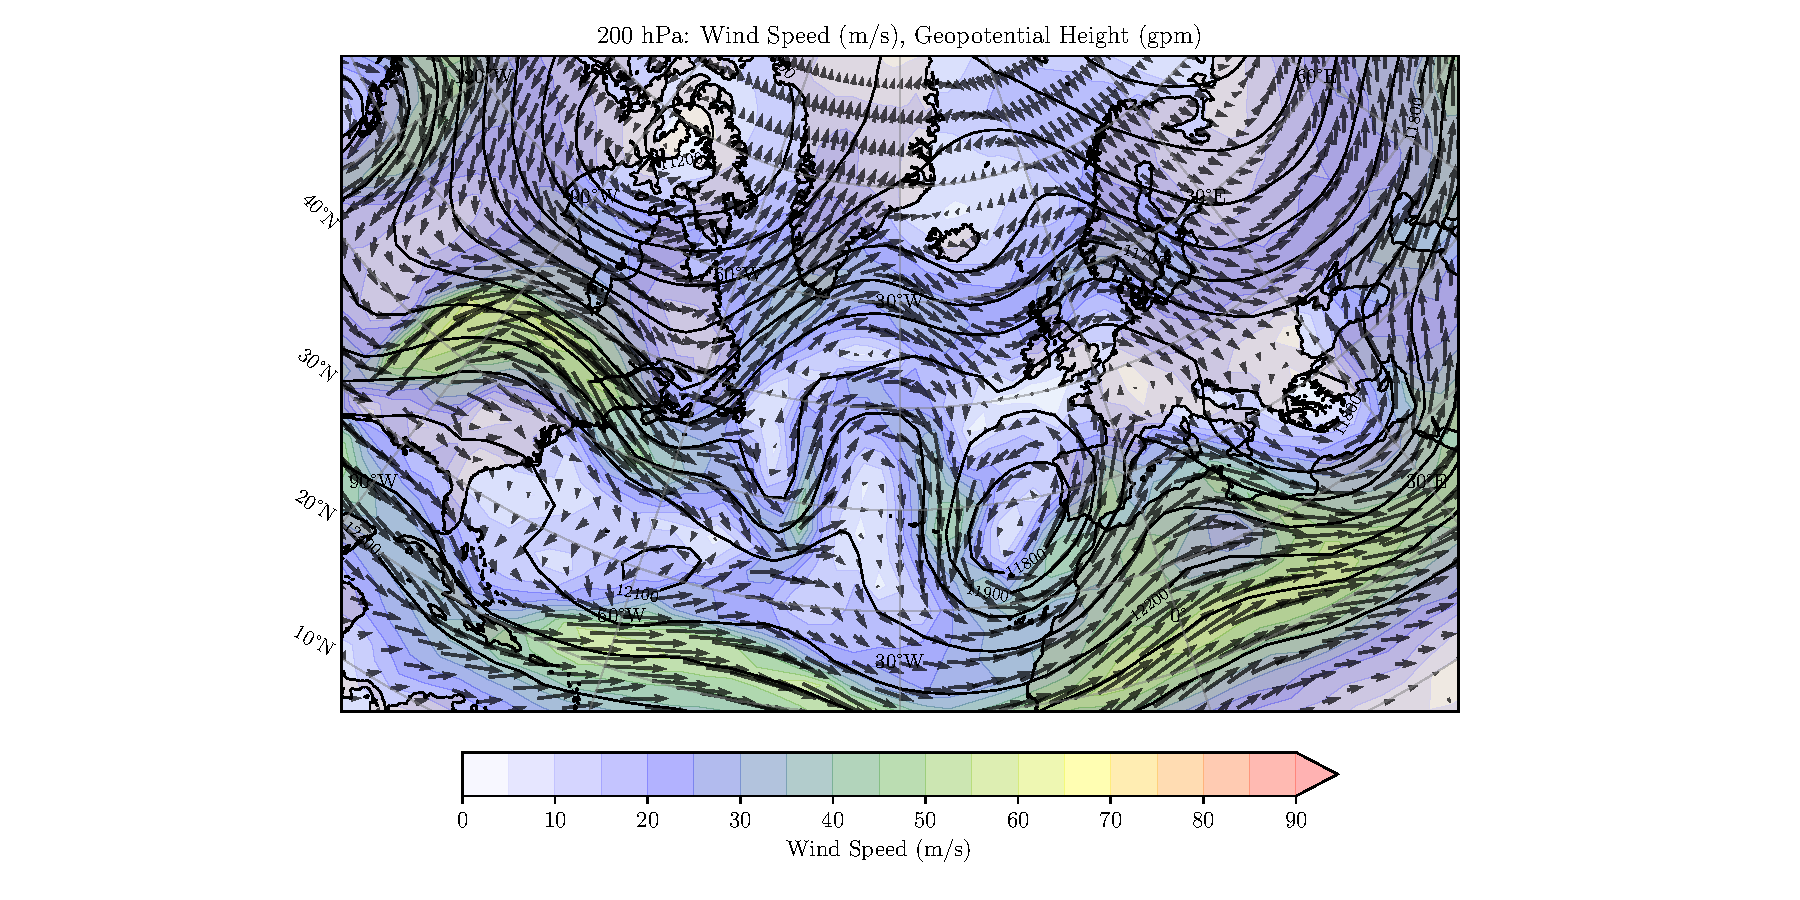
\includegraphics[width=\textwidth]{../images/weather/data_2025_5_1_00:00_200.pdf}
% \end{frame}

% % In your document body:
% \foreach \level in {850,500,200} {
% \foreach \day in {1,...,10} {
%   \foreach \time in {00:00,12:00} {
%       \begin{frame}
%         \frametitle{Forecast: \day-May-2025 at \time, Level \level hPa}
%         \includegraphics[width=\textwidth]{../images/weather/data_2025_5_\day_\time_\level.png}
%       \end{frame}
%     }
%   }
% }

% % In your document body:
% \foreach \level in {850,500,200} {
% \foreach \day in {1,...,10} {
%   \foreach \time in {00:00,12:00} {
%       \begin{frame}
%         \frametitle{Forecast: \day-May-2025 at \time, Level \level hPa}
%         \begin{center}
%           \includegraphics[width=0.5\textwidth]{../images/weather/data_2025_5_\day_\time_\level_polar.png}
%         \end{center}
%       \end{frame}
%     }
%   }
% }

% \foreach \n in {01,02,03,04,05,06,07,08,09,10,
%                 11,12,13,14,15,16,17,18,19,20,
%                 21,22,23,24,25,26,27,28,29,30,
%                 31} {
%   \begin{frame}
%     \begin{center}
%       \includegraphics[width=0.5\textwidth]{../images/rotating_earth/fig_\n.pdf}
%     \end{center}
%   \end{frame}
% }


% \begin{frame}
%   \frametitle{The Beta Plane Approximation}
%   \begin{itemize}
%     \item The beta plane approximation simplifies the Coriolis parameter \( f \) as:
%       \[
%       f = f_0 + \beta y
%       \]
%       where:
%       \begin{itemize}
%         \item \( f_0 \): Coriolis parameter at a reference latitude.
%         \item \( \beta \): Rate of change of \( f \) with latitude (\( \beta = \frac{\partial f}{\partial y} \)).
%         \item \( y \): Northward distance from the reference latitude.
%       \end{itemize}
%     \item Assumes small deviations from the reference latitude.
%     \item Useful for studying large-scale atmospheric and oceanic flows.
%   \end{itemize}
% \end{frame}
\begin{frame}
  \frametitle{Tilted Earth with 3D Spin}
  \begin{center}
    \begin{tikzpicture}[scale=1]
      % Tilted group (Earth and axes)
      \begin{scope}[rotate around={23.5:(0,0)}]
        % Axes
        \draw (-2,0) -- (2,0);
        \draw[->] (0,-2) -- (0,2) node[above] {$Pole$};

        % Earth (circle)
        \draw[thick] (1,0) arc[start angle=0, end angle=360, radius=1];

        % 3D-style spinning arrow (elliptical path)
        \draw[->, thick] ({0.3*cos(10)},{1.5 + 0.1*sin(10)})
        arc[start angle=10, end angle=320, x radius=0.3, y radius=0.1];
        % Point on the circle
        % \fill[red] ({cos(20)}, {sin(20)}) circle[radius=0.05] node[below right] {$P$};
        \fill[red] (30:1) circle[radius=0.05] node[right] {$P$};
        \draw[blue, thick] ($(30:1) + (120:0.5)$) -- ($(30:1) + (-60:0.5)$);
      \end{scope}
    \end{tikzpicture}
  \end{center}
\end{frame}

